% lecture notes by Umut Özer
% course: gr
\lhead{Lecture 14: November 13}
We will look at diffeomorphism of the action. However, the action does not depend on coordinates we use; the change of coordinates is like a gauge theory of the action. Similarly to Noether's theorem, where symmetries give rise to conserved quantities, this gauge symmetry will give rise to something. We will try to find out what that something is.

\begin{claim}
  Acting with an infinitesimal diffeomorphism along a vector field $X \in \mathfrak{X}(\mathcal{M})$, the metric changes as the Lie derivative
  \begin{equation}
    \delta g_{\mu\nu} = (\mathcal{L}_X g)_{\mu\nu}.
  \end{equation}
\end{claim}
\begin{proof}
  Consider a diffeomorphism that take points $x^{\mu}$ to nearby points $\widetilde{x}^{\mu}$ as
  \begin{equation}
    x^{\mu} \to \widetilde{x}^{\mu}(x) = x^{\mu} + \delta x^{\mu}.
  \end{equation}
  We also know that a vector field on a manifold induces a flow; we will use this to take us to this nearby point.
  As such, we can think of the associated coordinate change as being generated by a vector field $X^{\mu} = -\delta x^{\mu}$.
  The metric transforms as
  \begin{equation}
    g_{\mu\nu}(x) \to \widetilde{g}_{\mu\nu}(\widetilde{x}) = \frac{\partial^{} x^{\rho}}{\partial \widetilde{x}^{\mu}} \frac{\partial^{} x^{\sigma}}{\partial \widetilde{x}^{\nu}} g_{\rho\sigma} (x).
  \end{equation}
  The Jacobian associated with the change of coordinate $\tilde{x}^{\mu} = x^{\mu} - X^{\mu}(x)$ can be inverted:
  \begin{equation}
    \frac{\partial^{} \tilde{x}^{\mu}}{\partial x^{\rho}} = \delta^{\mu}_{\rho} - \partial_{\rho} X^{\mu} \quad \implies \quad \frac{\partial^{} x^{\rho}}{\partial \tilde{x}^{\mu}} = \delta^{\rho}_{\mu} + \partial_{\mu} X^{\rho} + \dots,
  \end{equation}
  where the higher order terms can be neglected for infinitesimal $X^{\mu}$.
  We then have
  \begin{align}
    \tilde{g}_{\mu\nu} (\tilde{x}) &= (\delta^{\rho}_{\mu} + \partial_{\mu} X^{\rho}) (\delta^{\sigma}_{\nu} + \partial_{\nu} X^{\sigma}) g_{\rho\sigma} (x) \\
				   &= g_{\mu\nu}(x) + g_{\mu\rho}(x) \partial_{\nu} X^{\rho} + g^{\nu\rho} (x) \partial_{\mu} X^{\rho}
  \end{align}
  Meanwhile, we may Taylor expand $\tilde{g}_{\mu\nu}(\tilde{x})$ on the left-hand side around $x$ to give
  \begin{equation}
  \widetilde{g}_{\mu\nu}(\tilde{x}) = \tilde{g}_{\mu\nu} (x + \delta x) = \widetilde{g}_{\mu\nu}(x) - X^{\lambda} \partial_{\lambda} g_{\mu\nu}(x).
  \end{equation}
  Thus, we find the change $\delta g_{\mu\nu}(x)$ of the metric at the point $x$ to be
  \begin{align}
    \delta g_{\mu\nu} \coloneqq \tilde{g}_{\mu\nu} (x) - g_{\mu\nu}(x) &= X^{\lambda} \partial_{\lambda} g_{\mu\nu} + g_{\mu\rho} \partial_{\nu} X^{\rho} + g_{\nu\rho} \partial_{\mu} X^{\rho} \\
	     &= (\mathcal{L}_X g)_{\mu\nu}.
  \end{align}
\end{proof}
Alternatively, we can write 
\begin{align}
  \delta g_{\mu\nu} &= \partial_{\mu} X_{\nu} + \partial_{\nu} X_{\mu} + X^{\rho}(\underbrace{\partial_{\rho} g_{\mu\nu} - \partial_{\mu} g_{\rho\nu} - \partial_{\nu} g_{\mu\rho}}_{2 g^{\rho\sigma} \Gamma^{\sigma}_{\mu\nu}})) \\
		    &= \nabla_{\mu} X_{\nu} + \nabla_{\nu} X_{\mu}.
\end{align}
Now look at the action
\begin{equation}
  \delta S = \int \dd[4]{x} \sqrt{-g} G^{\mu\nu} \delta g_{\mu\nu}.
\end{equation}
The symmetries of the action are those for which the change in the action is zero.
If we restrict to these changes of coordinates, it must be that for all choices of $X_{\nu}$, we have
\begin{equation}
  \dots = 2 \int \dd[4]{x} \sqrt{-g} G^{\mu\nu} \nabla_{\mu} X_{\nu} = 0
\end{equation}
because changing coordinates is a gauge symmetry.
Integrating by parts, and using the divergence theorem,
\begin{align}
  \dots &= -2 \int \dd[4]{x} \sqrt{-g} (\nabla_{\mu} G^{\mu\nu}) X^{\nu} \\
  \implies \nabla^{\mu} G_{\mu\nu} &= 0.
\end{align}
But we know that this is true for any metric. This is the Bianchi identity.
This is essentially another derivation of the Bianchi identity using the path integral, using the diffeomorphism invariance of the action.
\begin{leftbar}
  \begin{remark}
    The metric only actually has 6 pieces of information in it. However, the Einstein equations $G_{\mu\nu} = 0$ are 10 equations. You might think that this over-determines the metric, but the Bianchi identity saves us.
    In other words: $\nabla_{\mu} G^{\mu\nu} = 0$ are 4 conditions, which mean that the Einstein equations $G_{\mu\nu} = 0$ are really only 6 equations, which is the right number to determine the metric $g_{\mu\nu}$.
  \end{remark}
\end{leftbar}

\section{Some Simple Solutions}%
\label{sec:some_simple_solutions}

There are three cases that we should consider, depending on the cosmological constant: zero, positive and negative.
We will spend a lot of time understanding the differences between these solutions. Even the solutions that look completely trivial---such as the one we will write down shortly---have interesting subtleties about them.

\subsection{\texorpdfstring{$\Lambda = 0$}{Zero cosmological constant}: Minkowski Spacetime}%
\label{sub:zero_cosmological_constant_minkowski_spacetime}

Need to solve $R_{\mu\nu} = 0$. The solution $g_{\mu\nu}$ is not allowed!
\begin{leftbar}
  \begin{remark}
    Usually, the simplest solution that solves a field theory is always $\phi = 0$. On geometrical grounds, it is obvious that the metric cannot vanish, since we have to have an inverse.
    Nonetheless, this restriction, that none of the eigenvalues cross zero, is a very weird constraint to put on a dynamical field.
    What this might be telling us is that the metric is not a fundamental field of nature; the metric might emerge.
    For example, the other case where a field like this pops up is in fluid mechanics.
    When we write down the Navier-Stokes equations, we do not want the energy-density to cross zero, since the approximations that lead to the fluid equations break down otherwise.
    There are lots of hints that gravity is like fluid mechanics.
  \end{remark}
  Note that there are infinitely many solutions of these. We are nowhere close to understanding the properties of the general solution.
\end{leftbar}
The simplest solution is \emph{Minkowski spacetime}.
\begin{equation}
  ds^2 = -dt^2 + d\vb{x}^2
\end{equation}

\subsection{\texorpdfstring{$\Lambda > 0$}{Positive Cosmological Constant}: De Sitter Spacetime}%
\label{sub:$lambda > 0$_positive_cosmological_constant_de_sitter_spacetime}

There are many solutions, many of them very hard to solve since these are coupled second order differential equations. We will look for solutions to $R_{\mu\nu} = \Lambda g_{\mu\nu}$ of the form
\begin{equation}
  \label{eq:14-metric}
  ds^2 = -f(r)^2 dt^2 + f(r)^{-2} dr^2 + r^2 (d\theta^2 + \sin^2(\theta) d\phi^2).
\end{equation}
We can compute $R_{\mu\nu}$ (using for example the curvature two-forms) to find 
\begin{align}
  R_{t t } &= -f^4 R_{rr} = f^3 (f'' + \frac{2f'}{r} + \frac{(f')^2}{f}) \\
  R_{\phi\phi} &= \sin^2\theta R_{\theta\theta} = (1 - f^2 - 2 ff' r) \sin^2\theta.
\end{align}
With $R_{\mu\nu} = \Lambda g_{\mu\nu}$, this becomes
\begin{align}
  \mu,\nu &= t t, r r \implies f'' + \frac{2 f'}{r} + \frac{(f')^2}{f} = -\frac{\Lambda}{f}   \\
  \mu, \nu &= \theta\theta, \phi\phi \implies 1 - 2 ff' r - f^2 = \Lambda r^2
\end{align}
Both equations are solved by
\begin{equation}
  f(r) = \sqrt{1 - \frac{r^2}{R^2}}, \qquad \text{with } R^2 = \frac{3}{\Lambda}.
\end{equation}
This is \emph{de Sitter spacetime} dS (or the \emph{static patch} of dS).
\begin{leftbar}
  \begin{remark}
    $r\in [0, R]$ but the metric appears to be singular at $r = R$.
  \end{remark}
\end{leftbar}
Let us now build up some intuition of what it is like to live in a universe determined by metric \eqref{eq:14-metric}.
We can look at geodesics. With $\sigma$ denoting proper time, and $\dot(\dots) = \dv[]{(\dots)}{\sigma}$, we have the action:
\begin{equation}
  S = \int \dd[]{\sigma} \left[ -f(r)^2 (\dot t)^2 + f(r)^{-2} (\dot r)^2 + r^2 (\dot \theta^2 + \sin^2 \theta \dot \phi^2) \right].
\end{equation}
Given an action it is really tempting to find the equations of motion. However, in this case this is the wrong thing to do; the right thing to do is to consider the symmetries.
There are two conserved quantities: 
\begin{align}
  \text{angular momentum} \qquad l &= \frac{1}{2} \frac{\partial^{} L}{\partial \dot \phi} = r^2 \sin^2\theta \dot \phi \\
  \text{energy} \qquad E &= -\frac{1}{2} \frac{\partial^{} L}{\partial \dot t} = f(r)^2 \dot t.
\end{align}
For the action without the square root, we should also enforce a constraint that tells us whether things are timelike, spacelike, or null.
For massive particles, we require that the trajectory is timelike. With $\theta$ being proper time, this means that the Lagrangian itself should be $-1$:
\begin{equation}
  -f^2 \dot t^2 + f^{-2} \dot r^2 + r^2 (\dot \theta^2 + \sin^2\theta \dot \phi^2) = -1.
\end{equation}
For spacelike or timelike trajectories, we would have $1$ or $0$ on the right hand side respectively.
Let us look for geodesics with $\theta = \pi/2$ and $\dot \theta = 0$. This is similar to the Kepler problem, where we say that angular momentum is conserved, so all the motion has to be in the plane normal to the angular momentum vector.
Having done this, we do not look at the equations of motion, but instead see that the constraint becomes
\begin{equation}
  \implies \dot r^2 + V_{\text{eff}} (r) = E^2,
\end{equation}
with
\begin{equation}
  V_{\text{eff}}(r) = \qty(1 + \frac{l^2}{r^2}) \left( 1 - \frac{r^2}{R^2} \right).
\end{equation}
Here our intuition of relativistic Newtonian mechanics starts to kick in.
This is the usual angular momentum barrier, illustrated in Figure~\ref{fig:angmombar}.
\begin{figure}[tbph]
  \centering
  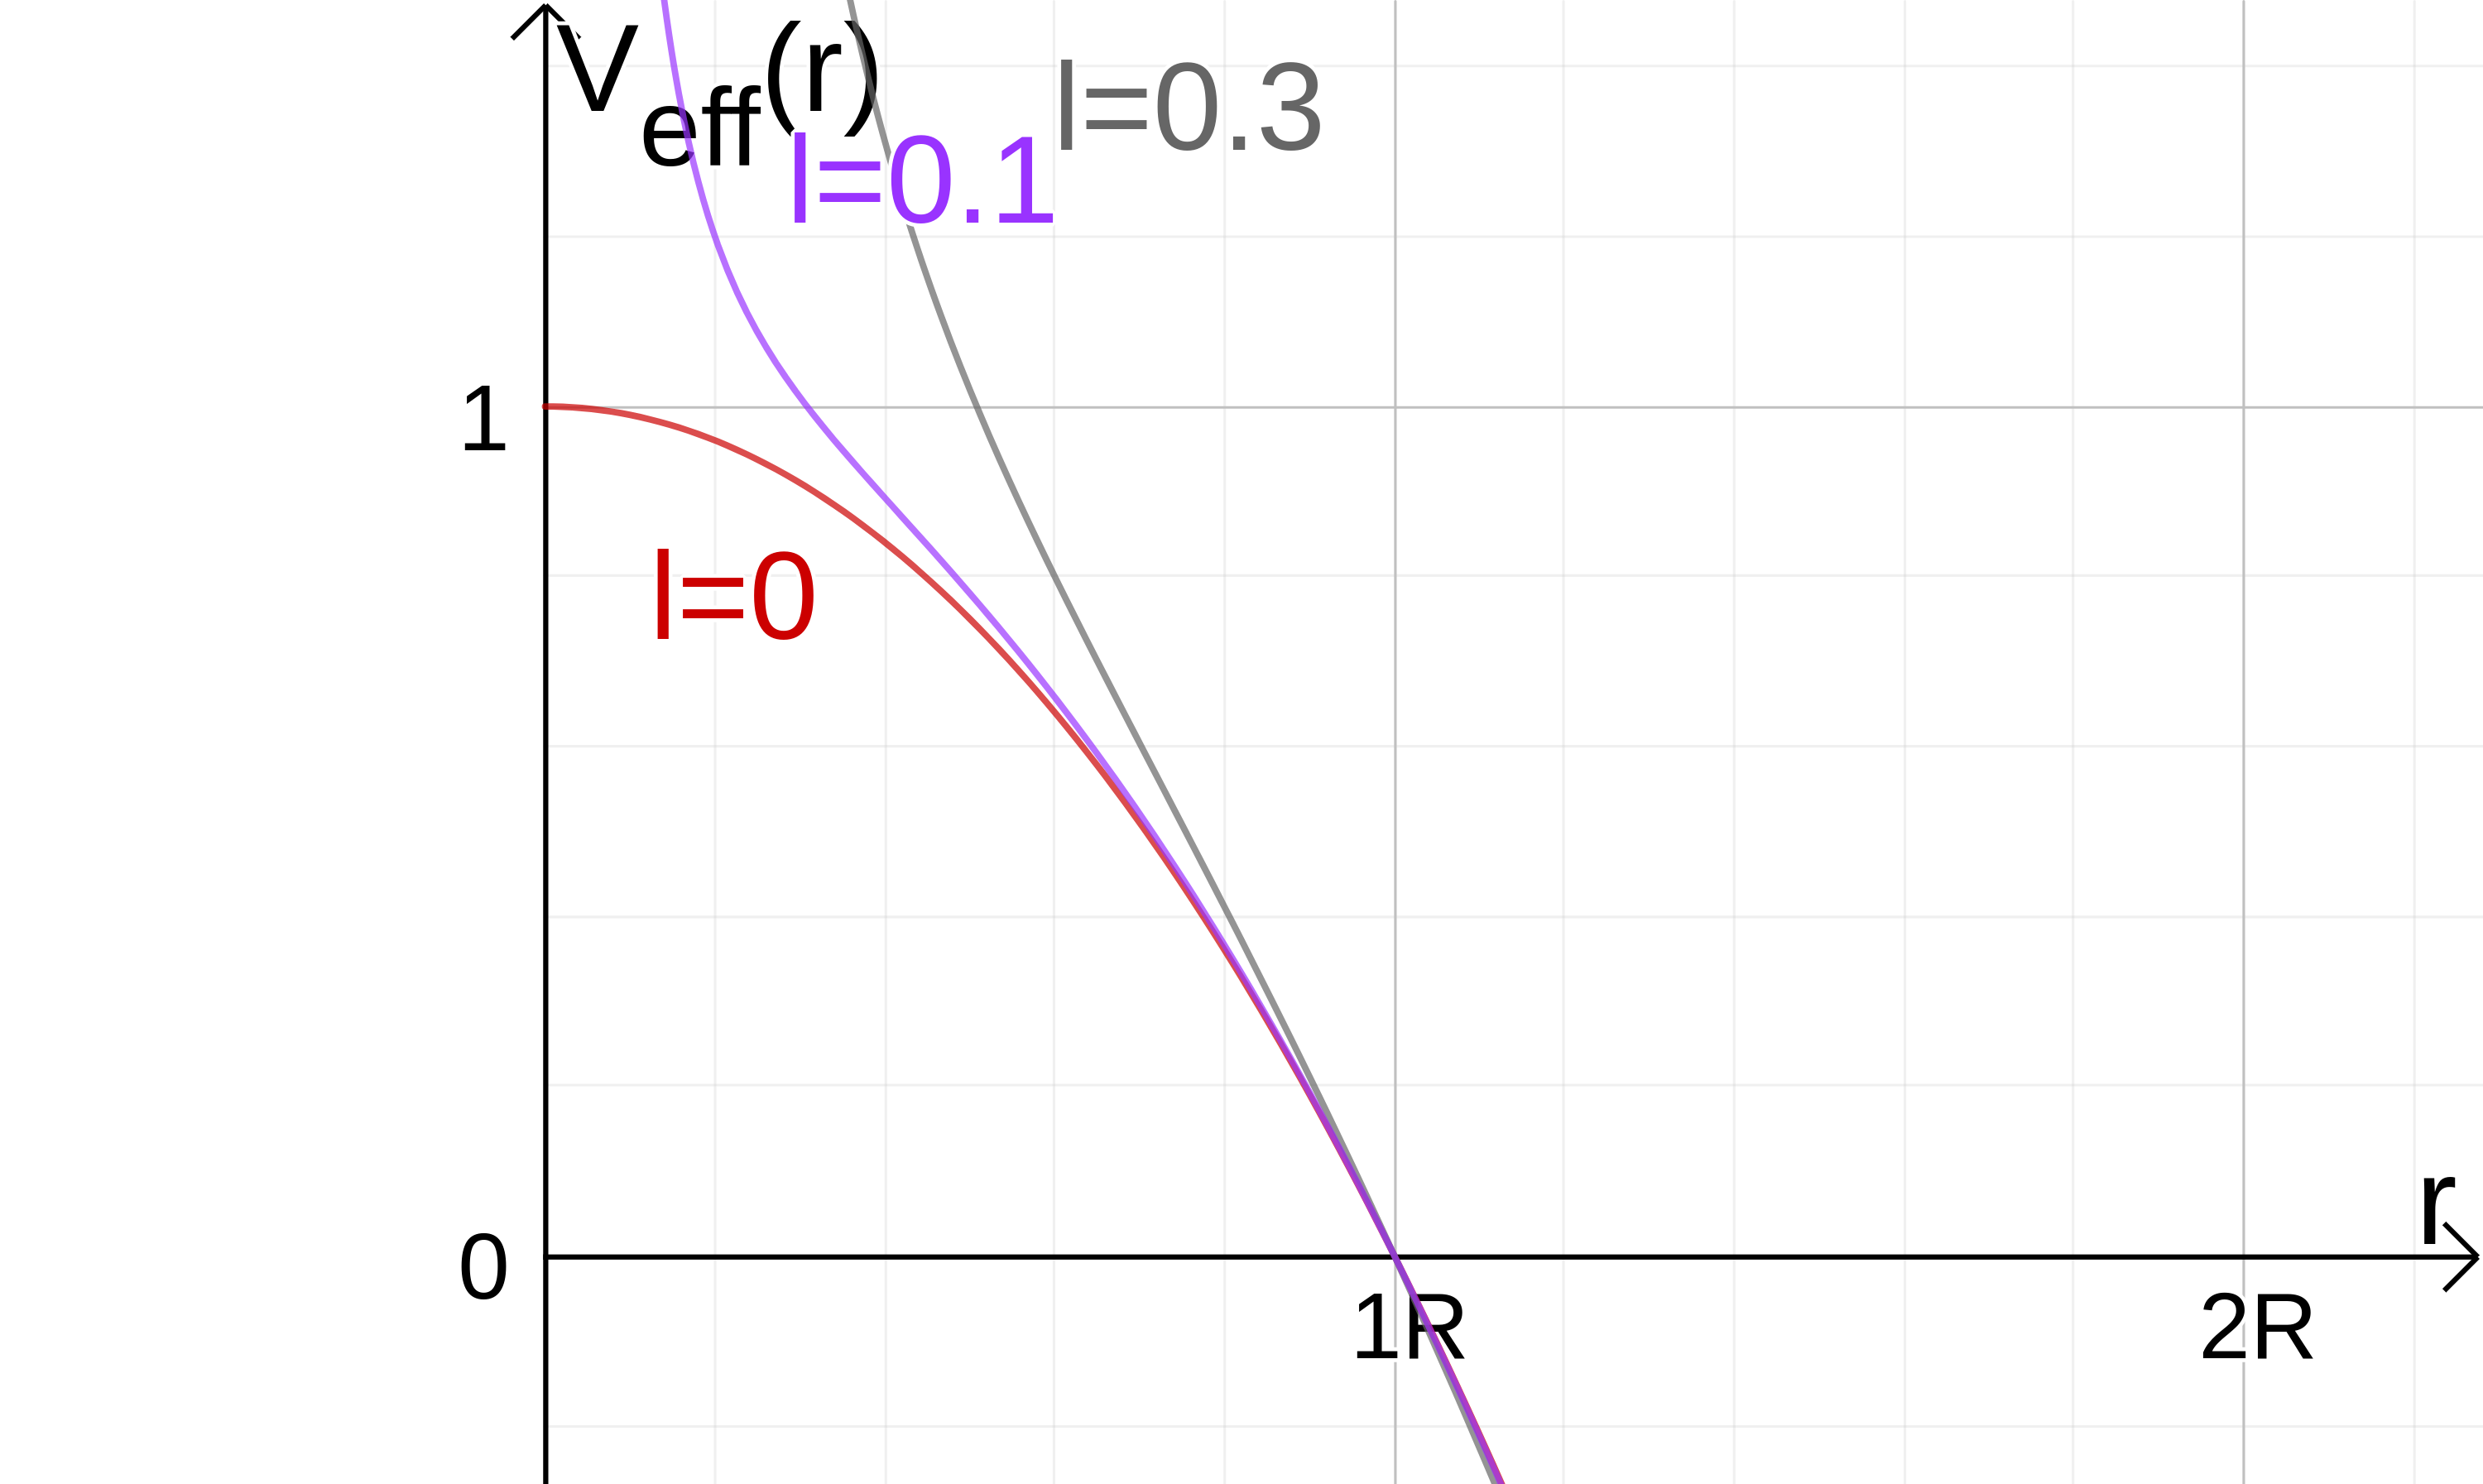
\includegraphics[width=0.6\columnwidth]{angmombar}
  \caption{}
  \label{fig:angmombar}
\end{figure}
Notice that the potential is unbounded from below, but it does so after the point at which we cannot trust the metric; it is singular at $r = R$ and so we should think of the particle to only be moving at $r < R$.
This is a bit like an inside-out black hole! We get pushed outwards.
For $l = 0$, we have
\begin{equation}
  r(\sigma) = R \sqrt{E^2 - 1} \sinh (\frac{\sigma}{R}).
\end{equation}
We can look for weird things that happen at the singularity $r = R$. However, nothing weird happens. In fact, this hits $r = R$ in some finite proper time $\sigma$. 
Meanwhile, we can ask what happens to coordinate time.
Coordinate time solves
\begin{equation}
  \dv[]{t}{\sigma} = E \left( 1 - \frac{r^2}{R^2} \right)^{-1}.
\end{equation}
\begin{claim}
  Solutions to this have $t \to \infty$ as $r \to R$.
\end{claim}
\begin{proof}
  To see this, suppose $r(\sigma_*) = R$ and expand $\sigma = \sigma_* - \epsilon$. Find that
  \begin{equation}
    \dv[]{t}{\epsilon} \approx - \frac{-\alpha}{\epsilon}
  \end{equation}
  for some constant $\alpha$.
  This implies that $t \sim -\alpha \log(\epsilon / R) \to \infty$ as $\epsilon \to 0$.
\end{proof}
This means that it takes a particle a finite proper time $\sigma$, but infinite coordinate time $t$, to move outwards from the origin and reach the singular point $r = R$.
\begin{leftbar}
  \begin{remark}
    Again, this looks very similar to an inside-out black hole.
    Ultimately, we will find out that this is where we live; our universe is like an inside-out black hole\dots
  \end{remark}
\end{leftbar}
